%!TEX root = ../bachelor.tex
\chapter{Fazit und Ausblick}
\label{ch:summary}

\section{Parallelisierung}
Der Kalibrierungsprozess sollte nur ein Mal durchgeführt werden müssen. Eine Parallelisierung bietet sich hier deshalb nur bedingt an. Man könnte jedoch 
\begin{itemize}
	\item Kalbirierungsprozess: Ransac, Hough
	\item sonst maps
\end{itemize}

\section{Verbesserung der Linien-Detektion}
Die Linien-Detektion basiert auf Hough-Transformationen und funktioniert nur mit relative homogenen Hintergründen. Darüber hinaus werden durch den aktuellen Ansatz sehr viele Linien detektiert, wobei anschließend die Schnittpunkte zwischen all diesen Kandidaten bestimmt werden müssen. Ein besserer Ansatz wäre die Gradientenrichtung des Kantenbilds miteinbeziehen. Dies reduziert die Anzahl falscher Votes und verbessert darüber hinaus die Laufzeit \cite{Gorman1976}. 


\section{Verbesserung der Vorwärtsentfaltung}
Das Hauptproblem der Vorwärtsentfaltung sind die Defekte auf dem entfalteten Bild. Man könnte mit Hilfe einer Delaunay-Triangulierung versuchen, die Defekte zu beheben. 
Die auf die Mantelfläche abgebildeten Punkte werden bei diesem Verfahren nicht gerundet. Anschließend werden die Punkte trianguliert. Es entstehen Dreiecksnetze, wie beispielhaft in Abbildung \ref{fig:delaunayTriag} zu sehen sind. Zum Zwecke der Veranschaulichung wurde hierbei nur ein Teil der Daten benutzt. Mit Hilfe dieser Dreiecke wird nun das Ergebnisbild abgetastet. Das heißt man untersucht für jedes Pixel auf dem entzerrten Bild in welchem Dreieck es sich befindet und bestimmt dann die Farbe des Pixels mittels baryzentrischer  Interpolation aus den drei umgebenden Punkten. Die Delaunay-Triangulierung ist jedoch relativ aufwendig mit einer Laufzeit von $\mathcal{O}(n\log n)$ für $n$ Punkte \cite{Su1997}. Sie richtet sich bei einer konstanten Eingabeauflösung also nach der Gesamtanzahl der Pixel im Kalibrierungskegel. Anschließend muss für jedes Pixel auf dem Ausgabebild eine Interpolation durchgeführt werden. Die Laufzeit der Vorwärtsentfaltung wird somit quadratisch mit einer großen additiven Konstante bedingt durch die Triangulierung.

\begin{figure}[!htb]
	\centering
	\begin{subfigure}{.9\textwidth}
		\centering
		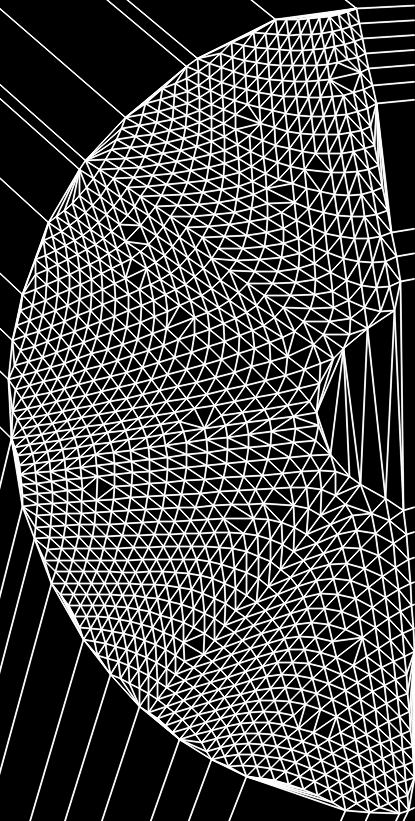
\includegraphics[angle=-90, width=.8\textwidth]{images/delaunay1.png}
		\caption{Triangulierung mit $10\%$ der Punkte}
	\end{subfigure}
	\begin{subfigure}{.9\textwidth}
		\centering
		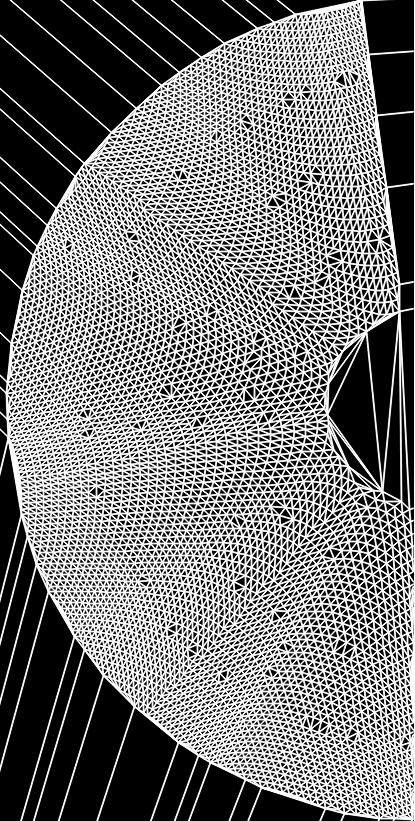
\includegraphics[angle=-90, width=.8\textwidth]{images/delaunay2.png}
		\caption{Triangulierung mit $40\%$ der Punkte}
	\end{subfigure}
	\caption{Delaunay-Triangulierung}
	\label{fig:delaunayTriag}
\end{figure}


\section{Verbesserung der Rückwärtsentfaltung}
Aktuell wird die Projektionsmatrix bei der Rückwärtsentfaltung durch \textit{Direct Linear Transformation} bestimmt. Dieses Verfahren minimiert jedoch nicht den Reprojektionsfehler. Besser wäre hier deshalb ein iteratives Verfahren, wie der Levenberg–Marquardt-Algorithmus (konkret für Projektionsmatrizen beschrieben in \cite{Hartley2000}).
Im Gegensatz dazu könnte auch ein RANSAC-Ansatz verwendet werden. Statt eine optimale Lösung für alle detektierte Samples zu bestimmen, berechnet man wiederholt für sechs Punkte\footnote{sechs Punkte sind mindestens notwendig um eine Projektionsmatrix bestimmen zu können, da es elf unbekannte gibt (siehe Kapitel \ref{s:calib}).} eine Projektionsmatrix und untersucht dann den Reprojektionsfehler für alle anderen Punkte und wählt schließlich die Projektionsmatrix mit dem größten Consensus Set aus. 


\section{Deformable Templates}
Energiefunktion ändern


\todo{Literatur überprüfen, insbesondere Seitenangaben}









